\documentclass{beamer}
\usetheme{ConnectivityLab}
\usepackage{times}
\usepackage{graphicx}
\usepackage{verbatim}
\usepackage{outlines}
\usepackage{fancyhdr}
\usepackage{subfigure}
\usepackage{cancel}
\usepackage{bibentry}
\usepackage{varwidth}
\usepackage{etoolbox}
\usepackage{epstopdf}

%%%%%%%%%%%%%%%%%%%%%%%%%%%%%%%%%%%%%%%%%%%%%%%%%%%%%%
%%%%%%%%%%%%%%%%%%%%%%%%%%%%%%%%%%%%%%%%%%%%%%%%%%%%%%

\title {
    SRUP: The Secure Remote Update Protocol\cite{eps402143}
}
\author {
    Speaker: Hsu, Yin-Hong
}
\date {
    01 10, 2017 %\today
}

%%%%%%%%%%%%%%%%%%%%%%%%%%%%%%%%%%%%%%%%%%%%%%%%%%%%%%
%%%%%%%%%%%%%%%%%%%%%%%%%%%%%%%%%%%%%%%%%%%%%%%%%%%%%%

\begin{document}
\begin{frame}
    \titlepage
\end{frame}

%%%%%%%%%%%%%%%%%%%%%%%%%%%%%%%%%%%%%%%%%%%%%%%%%%%%%%
%%%%%%%%%%%%%%%%%%%%%%%%%%%%%%%%%%%%%%%%%%%%%%%%%%%%%%

\begin{frame}{Outline}
    \tableofcontentsgather
    \tableofcontents
\end{frame}

%%%%%%%%%%%%%%%%%%%%%%%%%%%%%%%%%%%%%%%%%%%%%%%%%%%%%%
%%%%%%%%%%%%%%%%%%%%%%%%%%%%%%%%%%%%%%%%%%%%%%%%%%%%%%
\section{Introduction}

%%%%%%%%%%%%%%%%%%%%%%%%%%%%%%%%%%%%%%%%%%%%%%%%%%%%%%
%%%%%%%%%%%%%%%%%%%%%%%%%%%%%%%%%%%%%%%%%%%%%%%%%%%%%%
\begin{frame}{C2 and software update for IOT}
    \begin{itemize}
        \item {Enable the devices to receive and react to messages pertaining to the device itself}
        \item {This enables a human-operator or autonomous agent to interact with the device remotely}
    \end{itemize}
\end{frame}

%%%%%%%%%%%%%%%%%%%%%%%%%%%%%%%%%%%%%%%%%%%%%%%%%%%%%%
%%%%%%%%%%%%%%%%%%%%%%%%%%%%%%%%%%%%%%%%%%%%%%%%%%%%%%
\begin{frame}{Software Update \\ in the Internet of Things}
    \begin{itemize}
        \item {data-driven software}
        \begin{itemize}
            \item[-] Application's behaviour is determined by a combination of software and data
        \end{itemize}
        \item {using this type of approach can potentially simplify  many routine software updates}
    \end{itemize}
\end{frame}

\begin{frame}{The challenge of remote software update}
    \begin{itemize}
        \item{IoT device often have their primary UI provided by a network connection}
        \item{it must be impossible for the update process to cause the device be unusable}
        \item{be able to track whether a particular device has been updated}
    \end{itemize}
\end{frame}

\begin{frame}{Software Update paradigm}
    \begin{itemize}
        \item{two means to initiate a software update}
        \begin{itemize}
            \item[-] pushing the software to the device
            \item[-] triggering the device to fetch the software update itself
        \end{itemize}
        \item{use the second approach according to the first one is insucure}
        \item{to monitor a known repo, waiting for an indication that updates are available}
    \end{itemize}
\end{frame}

\begin{frame}{Cryptograph Security Considerations}
    \begin{itemize}
        \item{the URL of data can be found, can be verified by TLS}
        \item{their content checked for integrity using a hashing function (SHA2)}
        \item{to monitor a known repo, waiting for an indication that updates are available}
    \end{itemize}
\end{frame}
%%%%%%%%%%%%%%%%%%%%%%%%%%%%%%%%%%%%%%%%%%%%%%%%%%%%%%
%%%%%%%%%%%%%%%%%%%%%%%%%%%%%%%%%%%%%%%%%%%%%%%%%%%%%%
\section{Publish/Subscribe MQTT}

%%%%%%%%%%%%%%%%%%%%%%%%%%%%%%%%%%%%%%%%%%%%%%%%%%%%%%
%%%%%%%%%%%%%%%%%%%%%%%%%%%%%%%%%%%%%%%%%%%%%%%%%%%%%%
\begin{frame}{MQTT}
    \begin{itemize}
        \item{a lightweight brokered publish/subscribe protocol}
        \item{message will routed via broker to subscriber while publisher issue a message}
        \item{this research use MOSQUITTO as broker}
        \begin{itemize}
            \item[-] implements the MQTT protocol v3.1 and v3.1.1
            \item[-] open source
        \end{itemize}
    \end{itemize}
\end{frame}

%%%%%%%%%%%%%%%%%%%%%%%%%%%%%%%%%%%%%%%%%%%%%%%%%%%%%%
%%%%%%%%%%%%%%%%%%%%%%%%%%%%%%%%%%%%%%%%%%%%%%%%%%%%%%
\section{SRUP}
\begin{frame}{SRUP}
    \begin{figure}[t]
        \centering
        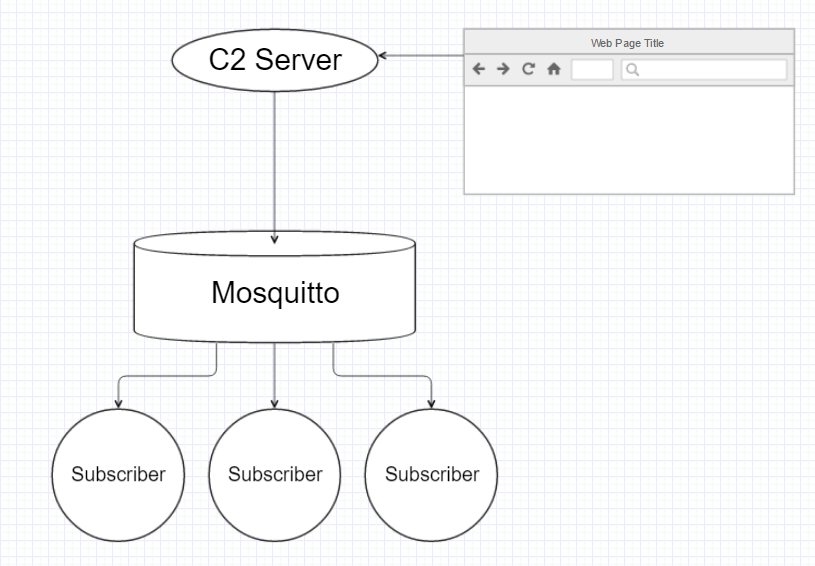
\includegraphics[width=0.9\textwidth]{figures/SRUP.png}
        \setbeamerfont{caption}{size=\tiny}
    \end{figure}
\end{frame}

\begin{frame}{SRUP}
    \begin{itemize}
        \item{although SRUP can be used in support of software updates on IoT devices, it is not a protocol for software updates}
        \item{SRUP does not attempt to provide a protocol for the actual download of the data but handled over a conventional HTTPS connection to the server providing the software}
        \item{previous version of the software would not be overwritten due to the purpose of recovery}
    \end{itemize}
\end{frame}

\begin{frame}{SRUP - advantage}
    \begin{itemize}
        \item{it makes it easy to target individual devices for specific updates}
        \item{provides a confirmable mechanism ensure that the update has been successfully and correctly received by device}
    \end{itemize}
\end{frame}

\begin{frame}{SRUP - action}
    \begin{figure}[t]
        \centering
        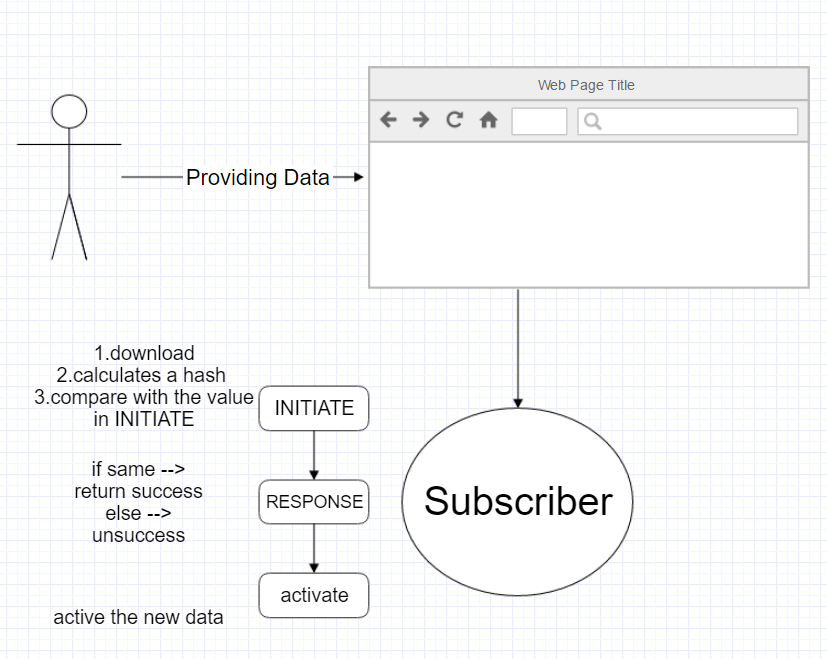
\includegraphics[width=0.9\textwidth]{figures/SRUP2.png}
        \setbeamerfont{caption}{size=\tiny}
    \end{figure}
\end{frame}

\section{Protocol detail}

\begin{frame}{Initiate MSG}
    \begin{figure}[t]
        \centering
        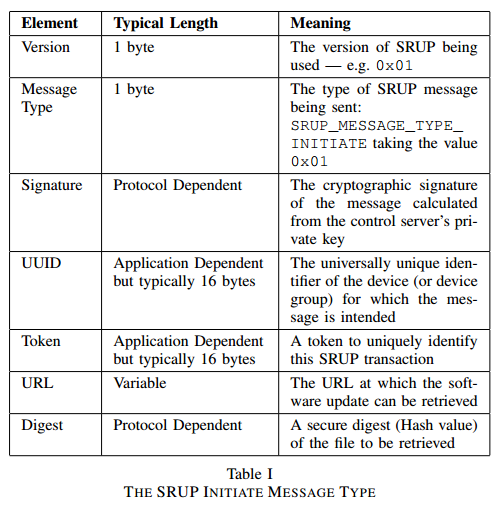
\includegraphics[width=0.7\textwidth]{figures/table1.png}
        \setbeamerfont{caption}{size=\tiny}
    \end{figure}
\end{frame}

\begin{frame}{Initiate MSG - example}
    \begin{figure}[t]
        \centering
        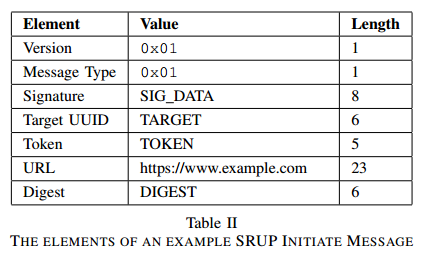
\includegraphics[width=0.9\textwidth]{figures/table2.png}
        \setbeamerfont{caption}{size=\tiny}
    \end{figure}
\end{frame}

\begin{frame}{Response MSG}
    \begin{figure}[t]
        \centering
        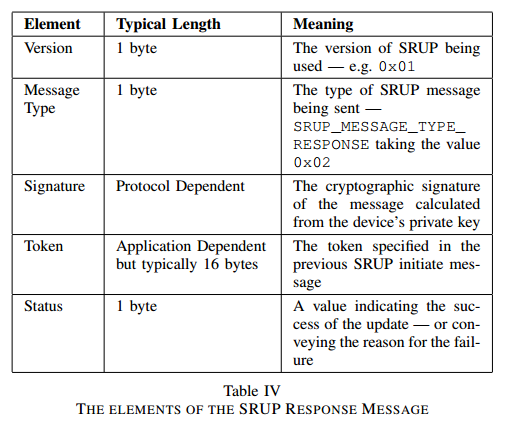
\includegraphics[width=0.7\textwidth]{figures/table4.png}
        \setbeamerfont{caption}{size=\tiny}
    \end{figure}
\end{frame}

\begin{frame}{Response MSG - example}
    \begin{figure}[t]
        \centering
        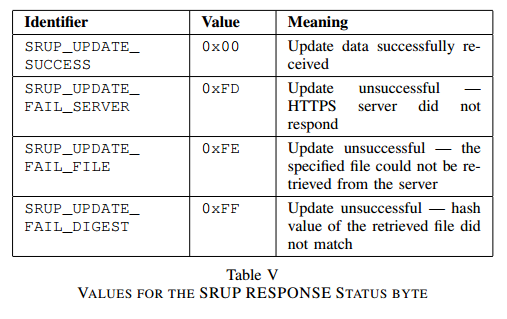
\includegraphics[width=0.9\textwidth]{figures/table5.png}
        \setbeamerfont{caption}{size=\tiny}
    \end{figure}
\end{frame}


\begin{frame}{Activatew MSG - example}
    \begin{figure}[t]
        \centering
        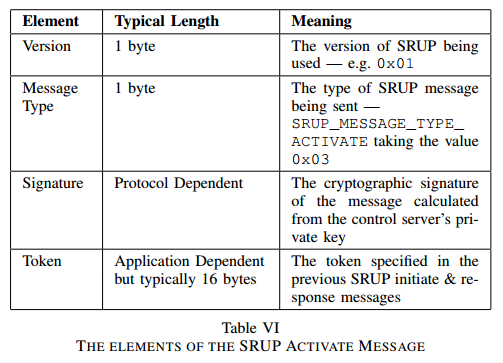
\includegraphics[width=0.9\textwidth]{figures/table6.png}
        \setbeamerfont{caption}{size=\tiny}
    \end{figure}
\end{frame}

\begin{frame}{SRUP - advantage}
    \begin{itemize}
        \item{it makes it easy to target individual devices for specific updates}
        \item{provides a confirmable mechanism ensure that the update has been successfully and correctly received by device}
    \end{itemize}
\end{frame}

%%%%%%%%%%%%%%%%%%%%%%%%%%%%%%%%%%%%%%%%%%%%%%%%%%%%%%
%%%%%%%%%%%%%%%%%%%%%%%%%%%%%%%%%%%%%%%%%%%%%%%%%%%%%%
\section{References}
\calcreferencespagetotal % Calc your References Page total number
\begin{frame}[allowframebreaks]{References}
    \fontsize{9pt}{13}\selectfont
    \bibliographystyle{IEEEtran}
    \bibliography{IEEEabrv,Citation}
\end{frame}

\section{}

\begin{frame}
    \centering
    \Large{Thanks for Your Attentions}
\end{frame}

\end{document}
